\begin{figure}[t]
\centering
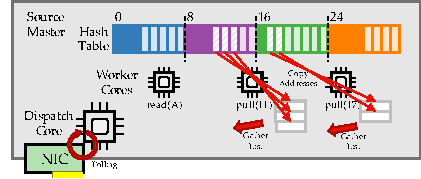
\includegraphics[width=0.9\columnwidth]{figures/rocksteady-source.pdf}
\caption{Source pull handling. \pulls work concurrently over disjoint
  regions of the source's hash table, avoiding synchronization, and
  return a fixed amount of data (20~KB, for example) to the target. Any
  worker core can service a \pull on any region, and all cores
  prioritize normal case requests over \pulls.}%
\label{fig:source}%
\end{figure}
